%!TeX root=../tese.tex
%("dica" para o editor de texto: este arquivo é parte de um documento maior)
% para saber mais: https://tex.stackexchange.com/q/78101/183146

%% ------------------------------------------------------------------------- %%
\chapter{Plataforma de Desenvolvimento}
\label{cap:plataforma de desenvolvimento}
\section{Estrutura Básica}

Quando se trata de desenvolvimento de jogos, o conceito de programação não pode se limitar aos tipos de programa \textquotedbl{\textit{batch mode}}\textquotedbl{}, isso é, programas que são executados em apenas duas etapas: o programador executa o programa; o programa devolve um resultado~\citep{IAEmTowerDefense}. Esse modelo é frequentemente usado, ainda mesmo nos dias atuais, para processamento de grandes volumes de dados, suportar reprodutibilidade, flexibilidade em termos de momento de execução, e geração de logs detalhados, entre outros cenários~\citep{BatchProgramming}.

Os programas interativos, por sua vez, compõem a estrutura dos jogos digitais como conhecidos atualmente. Este modelo, por sua vez, se resume ao pequeno bloco de código a seguir.

\begin{program}
    \lstinputlisting[
      language=pseudocode,
      style=pseudocode,
      style=wider,
      functions={},
      specialidentifiers={},
    ]
    {conteudo/gameloop.py}
  
    \caption{Game Loop\label{prog:gameloop}}
\end{program}

Essa estrutura é conhecida como \textit{Game Loop}~\citep{GameProgramming}. O jogo primeiramente processa o input recebido pelo usuário, atualiza as variáveis do jogo de acordo e, finalmente, desenha os resultados na tela. Este pequeno trecho de código é projetado para ser executado, idealmente, um total de 60 vezes por segundo, em intervalos de tempos iguais, gerando a denominada \textit{frame}\footnote{
    Um \textquotedbl{quadro}\textquotedbl{} do jogo. A rápida sequência de quadros gerados pelo \textit{game loop} resulta na animação geral do jogo.
}. Com isso, cada \textit{frame} do jogo será apresentada apenas durante aproximadamente 0.016 segundos até ser substituída pela próxima pelo código do \textit{Game Loop}.

Por uma questão de simplicidade e para eliminar a necessidade de recriar essa estrutura para qualquer programa interativo, \textit{frameworks} dedicadas para o desenvolvimento desse tipo de programa tornaram-se disponíveis, mais especificamente para o cenário de desenvolvimento de jogos, as \textit{Game Engines}\footnote{
    Alguns exemplos de \textit{engines} famosas hoje em dia: Unity; Unreal Engine; CryEngine; GameMaker Studio; RPG Maker; Godot.
}. Também conhecidas como \textit{Motor de Jogo}, essas auxiliam fortemente no desenvolvimento tanto jogos 2D quanto 3D, além de uso de gráficos, audio, bancos de dados, físicas, ou até mesmo uso de outras \textit{frameworks} para, por exemplo, comunicação entre redes. A \textit{engine} utilizada para desenvolver o protótipo neste estudo foi a \textit{Godot Engine}.

\section{Sobre a Godot Engine}

A \textit{Godot Engine} é uma \textit{engine} totalmente gratuita e \textit{open-source} sob a licença MIT, dedicada para o desenvolvimento de aplicativos 2D ou 3D, principalmente jogos eletrônicos, e tem sua manutenção feita atualmente pela comunidade de forma independente. A versão da engine utilizada neste estudo foi a 3.2.3, parte da versão 3.0 da \textit{Godot}, lançada em 2018. Para entendimento do protótipo desenvolvido e do estudo feito, esta seção será dedicada a explicar os elementos básicos da \textit{engine}, assim como algumas funcionalidades adicionais.

Falar esse finalzinho? numsei

\subsection{Nós}

Também conhecidos como \textit{Nodes}, quando separados, representam pequenos elementos do jogo. Quando juntos, compoem a estrutura geral do jogo, como blocos de construção. Na \textit{Godot}, exitem diversos tipos diferentes de nós, cada um com uma função específica, e possivelmente herdando funcionalidades de outros tipos de nós. Por outro lado, os nós por padrão terão as seguintes utilidades:

\begin{itemize}
    \item Possuem um nome
    \item Possuem atributos (variáveis)
    \item Podem possuir ou não um trecho de código que é chamado toda \textit{frame} do jogo, definido em um \textit{script}
    \item Podem possuir ou não métodos customizados, definidos no \textit{script} mencionado
    \item Podem herdar funcionalidades de outros nós ou scripts criados
    %(tendo assim atributos e métodos de ambos scripts, o atribuído e o herdado)
    \item Podem ser inseridos como \textit{filhos} de outros nós, compondo uma \textit{cena}
    %, herdando \textquotedbl{forçadamente}\textquotedbl{} atributos como posição na tela
\end{itemize}

Usufruindo de todas essas funções, o desenvolvimento do jogo é focado quase totalmente no uso dos nós.

\begin{figure}
    \centering

    \begin{subfigure}{.9\textwidth}
        \centering
        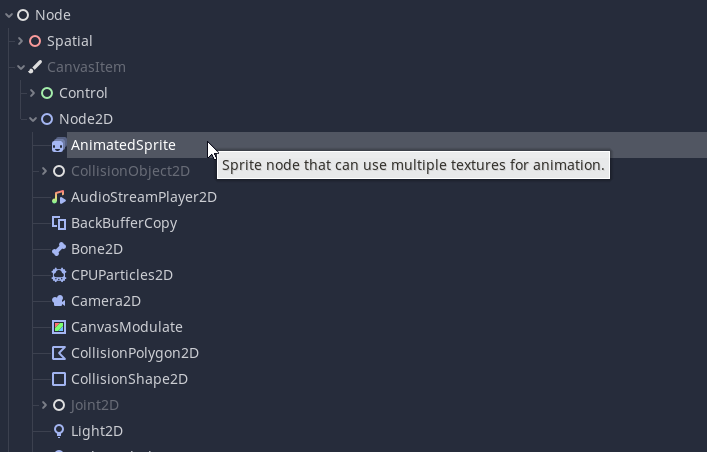
\includegraphics[width=1\textwidth]{tiposDeNos}
    \end{subfigure}

    \caption{Tela de criação de \textit{novo nó}, dentro da \textit{Godot}}
\end{figure}

\subsection{Cenas}

Como mencionado anteriormente em~\ref{Cenas}, uma cena pode representar não apenas um estado específico do jogo, como um determinado \textquotedbl{objeto}\textquotedbl{}, por exemplo, o personagem principal ou um inimigo. Cenas são sempre compostas por um ou mais nós em uma estrutura de árvore.

\begin{figure}
    \centering

    \begin{subfigure}{.4\textwidth}
        \centering
        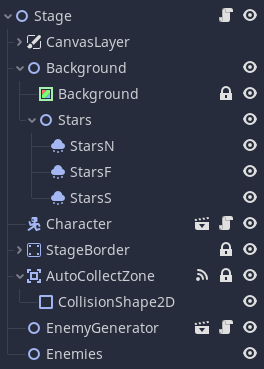
\includegraphics[width=1\textwidth]{arvoreDeNos}
    \end{subfigure}

    \caption{Árvore de nós da cena principal do jogo}
\end{figure}